\chapter{Implementing Egress and Ingress Scenarios Using Selected CNI Plugins}
\label{cha:practical_impl}

This chapter presents the implementation of egress and ingress scenarios. The egress scenario will be executed locally, while the ingress scenario will be deployed both on local infrastructure (personal laptop) and on the public cloud (Azure). The tools used in this implementation with some example configurations will be described.
The Kubernetes cluster will run on a local laptop with the following specifications:
\begin{itemize}
  \item CPU: AMD Ryzen 5 3500U 8 CPUs
  \item RAM: 20 GB
  \item Storage: 256 GB SSD
  \item Operating System: Fedora 40 with kernel 6.10.11
\end{itemize}

Cloud infrastrucure consist of two AKS nodes (virtual machines) of type Azure Standard\_A2\_v2. Each VM has the following specifications:
\begin{itemize}
  \item CPU: 2 vCPUs
  \item RAM: 4 GB
  \item Storage: Standard SSD
  \item Operating System: Ubuntu 22.04
\end{itemize}




%---------------------------------------------------------------------------


\section{Tools and automation}
\label{sec:tools}

In this section, the tools used to provision the egress and ingress implementations will be described. A Kubernetes cluster will be created to simulate the scenarios, and Infrastructure as Code (IaC) tool Terraform will be used to provision and interact with the cluster. Additionally, Ansible will be used for creating, configuring cluster setups along with running terraform and performance tools.


%---------------------------------------------------------------------------

\subsubsection{Ansible}
\label{sec:ansible}

Ansible is an opensource tool which is able to automate provisioning and configuring infrastructure. Configuration in Ansible is written in playbooks, which are YAML files as blueprints that contain a set of instructions to be executed. Each playbook consists of one or more plays, and each play describes a set of tasks to be performed on a group of desired hosts \cite{Ansible} \cite{AnsiblePlaybook}.

\begin{listing}[htb]
    \centering
    \caption{Example ansible playbook \cite{AnsibleOpenstack}.}
    \begin{minted}[gobble=4, frame=single, linenos, fontsize=\scriptsize]{yaml}
    - name: Create openstack instance and assign floating ip
      hosts: "{{ openstack_pool | default('localhost') }}"
      var_files:
        - ./vars/auth.yml
      become: yes
  
      tasks:
        - name: Create the OpenStack instance
          openstack.cloud.server:
            state: present
            name: " {{ inventory_hostname }}"
            key_name: "{{ key_name }}"
            network: "{{ network_name }}"
            auth:
              auth_url: "{{ auth_url }}"
              username: "{{ username }}"
              password: "{{ password }}"
              project_name: "{{ project_name }}"
  
      roles:
        - assign_floating_ip

    \end{minted}
    \label{lst:exampleAnsiblePlaybook}
\end{listing}

\begin{listing}[htb]
    \centering
    \caption{Example ansible inventory \cite{AnsibleInventory} \cite{AnsibleOpenstack} \cite{AnsibleVars}}
    \begin{minted}[gobble=4, frame=single, linenos, fontsize=\scriptsize]{yaml}
    [openstack_pool]
    instance-1.example.com key_name=ansible_key network_name=my-network ansible_host=10.10.10.10
    instance-2.example.com key_name=ansible_key network_name=my-network ansible_host=10.10.10.20
    \end{minted}
    \label{lst:exampleAnsibleInventory}
\end{listing}


Listing~\ref{lst:exampleAnsiblePlaybook} shows example ansible playbook configuration. Hosts field define group of objects on which configuration script is executed. In this case instances specified in group named openstack\_pool in ansible inventory showed on listing~\ref{lst:exampleAnsibleInventory} will be created when using the playbook. Using var\_files is possible to attach file containg, for example authentication variables required to access openstack cloud. Become is used to execute script as root user. Tasks and roles is the place, where actual script is defined. It can be defined directly in tasks, or specified by a roles, in this case will use script from ./roles/assign\_floating\_ip/tasks/main.yaml \cite{AnsiblePlaybook}.


\subsubsection{Iperf3}
\label{sec:iperf3}

Iperf3 is a tool capable of measure networking metrics. It supports TCP, UDP and SCTP protocols in IPv4 or IPv6 networks. The tool works in client-server architecture. Iperf3 will be used to evalutate throughput and round trip time in egress scenario. Listings~\ref{lst:iperfServer} and~\ref{lst:iperfClient} shows how to run iperf three seconds measurement within localhost interface \cite{Iperf}.

\begin{listing}[H]
    \centering
    \caption{Running iperf3 server command \cite{IperfDocs}.}
    \begin{minted}[gobble=4, frame=single, linenos, fontsize=\scriptsize]{bash}
    $ iperf3 --server
    -----------------------------------------------------------
    Server listening on 5201 (test #1)
    -----------------------------------------------------------
    Accepted connection from 127.0.0.1, port 40496
    [  5] local 127.0.0.1 port 5201 connected to 127.0.0.1 port 40502
    [ ID] Interval           Transfer     Bitrate
    [  5]   0.00-1.00   sec  5.55 GBytes  47.6 Gbits/sec                  
    [  5]   1.00-2.00   sec  5.97 GBytes  51.3 Gbits/sec                  
    [  5]   2.00-3.00   sec  5.50 GBytes  47.3 Gbits/sec                  
    [  5]   3.00-3.00   sec  4.50 MBytes  38.7 Gbits/sec                  
    - - - - - - - - - - - - - - - - - - - - - - - - -
    [ ID] Interval           Transfer     Bitrate
    [  5]   0.00-3.00   sec  17.0 GBytes  48.7 Gbits/sec                  receiver
    \end{minted}
    \label{lst:iperfServer}
\end{listing}

\begin{listing}[H]
    \centering
    \caption{Running iperf3 client command \cite{IperfDocs}.}
    \begin{minted}[gobble=4, frame=single, linenos, fontsize=\scriptsize]{bash}
    $ iperf3 --client 127.0.0.1 --time 3
    Connecting to host 127.0.0.1, port 5201
    [  5] local 127.0.0.1 port 40502 connected to 127.0.0.1 port 5201
    [ ID] Interval           Transfer     Bitrate         Retr  Cwnd
    [  5]   0.00-1.00   sec  5.55 GBytes  47.6 Gbits/sec    0   1.31 MBytes       
    [  5]   1.00-2.00   sec  5.97 GBytes  51.3 Gbits/sec    0   1.50 MBytes       
    [  5]   2.00-3.00   sec  5.50 GBytes  47.2 Gbits/sec    0   1.50 MBytes       
    - - - - - - - - - - - - - - - - - - - - - - - - -
    [ ID] Interval           Transfer     Bitrate         Retr
    [  5]   0.00-3.00   sec  17.0 GBytes  48.7 Gbits/sec    0             sender
    [  5]   0.00-3.00   sec  17.0 GBytes  48.7 Gbits/sec                  receiver

    iperf Done.
    \end{minted}
    \label{lst:iperfClient}
\end{listing}

\subsubsection{Kind}
\label{sec:kind}

Kind is a tool used for creating local Kuberentes cluster. This tool can simulate real communication between nodes within one machine. It creates control plane and worker nodes using Docker containers to enable node to node communication. The important thing is that it does not provide any load balancer for assigning external IP addresses for Kubernetes services. In ingress scenario Gateway API requires outside cluster routable IP address, on local infrastructure MetalLB will be installed and configured to provide IPs \cite{Kind}. Listing~\ref{lst:kindConfig} shows kind configuration used in both egress and ingress scenation on local infrastructure. One control plane node and two worker nodes are created. It also disables default CNI plugin which is essentail in this case.

\begin{listing}[H]
    \centering
    \caption{Kind config used in both scenarios \cite{KindConfig}.}
    \begin{minted}[gobble=4, frame=single, linenos, fontsize=\scriptsize]{yaml}
    kind: Cluster
    apiVersion: kind.x-k8s.io/v1alpha4
    networking:
        disableDefaultCNI: true
    nodes:
        - role: control-plane
          extraPortMappings:
            - containerPort: 80
              hostPort: 80
            - containerPort: 443
              hostPort: 443
        - role: worker
        - role: worker
    \end{minted}
    \label{lst:kindConfig}
\end{listing}

\subsubsection{K6}
\label{sec:k6}

Grafana K6 is open-source tool designed for load testing by simulating virtual users accessing specified endpoints. The testing configuration is written in a JavaScript file using the k6 library. Listing~\ref{lst:k6Config} demonstrates k6 script used in the ingres scenario. It is written as an Ansible template. During the ingress test Ansible injects variables into the script, allowing k6 to probe the Gateway API \cite{AnsibleTemplates}.


\begin{listing}[H]
  \centering
  \caption{Grafana k6 script used in the infress scenario \cite{K6HTTP}.}
  \begin{minted}[gobble=4, frame=single, linenos, fontsize=\scriptsize]{javascript}
    import http from 'k6/http';

    export const options = {
      vus: "{{ number_of_vusers }}",
      duration: "{{ test_duration }}s",
    };

    export default function () {
        const timestamp = new Date().toISOString();

        const res = http.get('http://{{ gateway_api_ip.stdout }}/echo');

        const hostnameMatch = res.body.match(/Hostname:\s*(\S+)/);
        const hostname = hostnameMatch ? hostnameMatch[1] : 'Hostname not found';

        console.log(`[${timestamp}] Hostname: ${hostname}`);
    }
  \end{minted}
  \label{lst:k6Config}
\end{listing}

\subsubsection{MetalLB}
\label{sec:metallb}

MetalLB is an implementation of load balancer for bare metal Kubernetes. Kind does not provide implementation of load balancer. Without external tool like this, load balancer type service will persist in "pending" state. It is mandatory in ingres scenario to create loadbalancing service (in this case to allocate external IP address) for Gateway API \cite{MetalLB}.

\subsubsection{Node Exporter}
\label{sec:nodeExporter}

A tool that exports the current system's metrics, such as CPU usage, memory utilization, disk I/O, and network statistics. The metrics in OpenMetrics format are exposed on /metrics enpoind \cite{NodeExporter}.

\subsubsection{Prometheus}
\label{sec:prometheus}

Prometheus is a monitoring and alerting tool, which stores data in time series, any data value is associated with time when it was collected. Stored data can be retrieved using PromQL (query language). The tool colects data by pulling from specified enpoints in configuration \cite{Prometheus}. 

\subsubsection{Terraform}
\label{sec:terraform}

Terraform is an open-source infrastructure as code (IaC) tool. It allows provision, and manage infrastructure resources, cloud infrastructure, kubernetes cluster, virtual machines, docker containers, storage and also SaaS features. Configuration files are written in a declarative language called HashiCorp Configuration Language (HCL).

The Terraform workflow is made up of three stages \cite{Terraform}:
\begin{enumerate}
  \item Write -- define in configuration file resources to be created
  \item Plan -- shows the actual resources that will be created based on the provided configuration and checks for any errors in the code
  \item Apply -- provision resources or applys changes defined in write stage to the infrastructure 
\end{enumerate}



%---------------------------------------------------------------------------


\section{Egress scenario implementation}
\label{sec:egressImpl}


The engress scenario compares Antrea and Cilium egress gateway implementation performance. The overall resource utilization will be evaluated by comparing the results of running the same test with and without redirecting traffic through the egress gateway. The test involves using iperf3 in TCP mode to measure network performance. The iperf3 is located in a pod inside Kubernetes cluster, on the other hand iperf server runs on personal computer which launches cluster. The network resources are collected by iperf3, and CPU/memory usage is monitored by a node exporter. These include:
\begin{itemize}
  \item CPU -- the processing power utilized by the cluster.
  \item Memory -- the amount of RAM consumed by the infrastructure.
  \item Throughput -- The volume of data successfully transmitted per unit of time.
  \item RTT (Round-Trip Time) -- The time taken for a data packet to travel to its destination and back.
\end{itemize}

%---------------------------------------------------------------------------
\subsection{Antrea}
\label{sec:antreaEgress}

In this part of the scenario, Antrea CNI is installed on a locally hosted Kubernetes cluster using Kind. An Ansible playbook automates the process by creating the cluster, installing the CNI, deploying the egress gateway, and running the test. The script used for this setup is shown below on listing ~\ref{lst:antreaEgressPlaybook}:

\begin{listing}[H]
  \centering
  \caption{Kind config used in both scenarios \cite{KindConfig}.}
  \begin{minted}[gobble=4, frame=single, linenos, fontsize=\scriptsize]{yaml}
    - name: Create antrea egress scenario with egress gateway
      hosts: "{{ target | default('localhost') }}"
      vars_files:
        - ./vars/antrea.yml
        - ./vars/common.yml
        - ./vars/egress_gateway.yml
        - ./vars/local.yml

      roles:
        - create_kind_cluster
        - install_antrea
        - wait_until_antrea_installed
        - get_ip_for_egress_node
        - deploy_antrea_egress_gateway
        - monitoring
        - terraform_run_egress_iperf
        - scrap_prometheus_data
  \end{minted}
  \label{lst:antreaEgressPlaybook}
\end{listing}

Four file containing variables included in the script:
\begin{enumerate}
  \item common.yml -- contains shared variables like ansible become password to access root privileges on machine
  \item egress\_gateway.yml -- scenario name or node name on which deploy gateway
  \item antrea.yml -- CNI name for later use, such as specifying the cluster name and the folder path where test results are stored
  \item local.yml -- informations about local infrastructure, like node names, job name for prometheus and env type
\end{enumerate}

The actual playbook from listing~\ref{lst:antreaEgressPlaybook} consist of eight steps to perform automate provisioning infrastructure, running test and store output:
\begin{enumerate}
  \item create\_kind\_cluster -- creates kind cluster using config presented on listing~\ref{lst:kindConfig}
  \item install\_antrea -- applies massive antrea yaml containing custom resource definitions which define cluster networking 
  \item wait\_until\_antrea\_installed -- uses kubectl wait command and stops script intil antrea controller deployment is available
  \item get\_ip\_for\_egress\_node -- retrieves ip address of node by name specified in variable files on which deploy egress gateway in the next step 
  \item deploy\_antrea\_egress\_gateway -- turns on egress support in Antrea CNI using config map and creates static egress gateway by setting egressIP field to previously obtained IP address 
  \item monitoring -- applies monitoring in cluster, deploys Prometheus Deployment and Node Exporter DaemonSet
  \item terraform\_run\_egress\_iperf -- runs iperf3 server on laptop, saves current timestamp and runs iperf3 client Pod using terraform.
  \item scrap\_prometheus\_data -- part of playbook responsible for pulling CPU and memory metrics stored by prometheus
\end{enumerate}

The playbook from listing~\ref{lst:antreaEgressPlaybook} produces following infrastructure:

\begin{figure}[tbh]
  \centering
  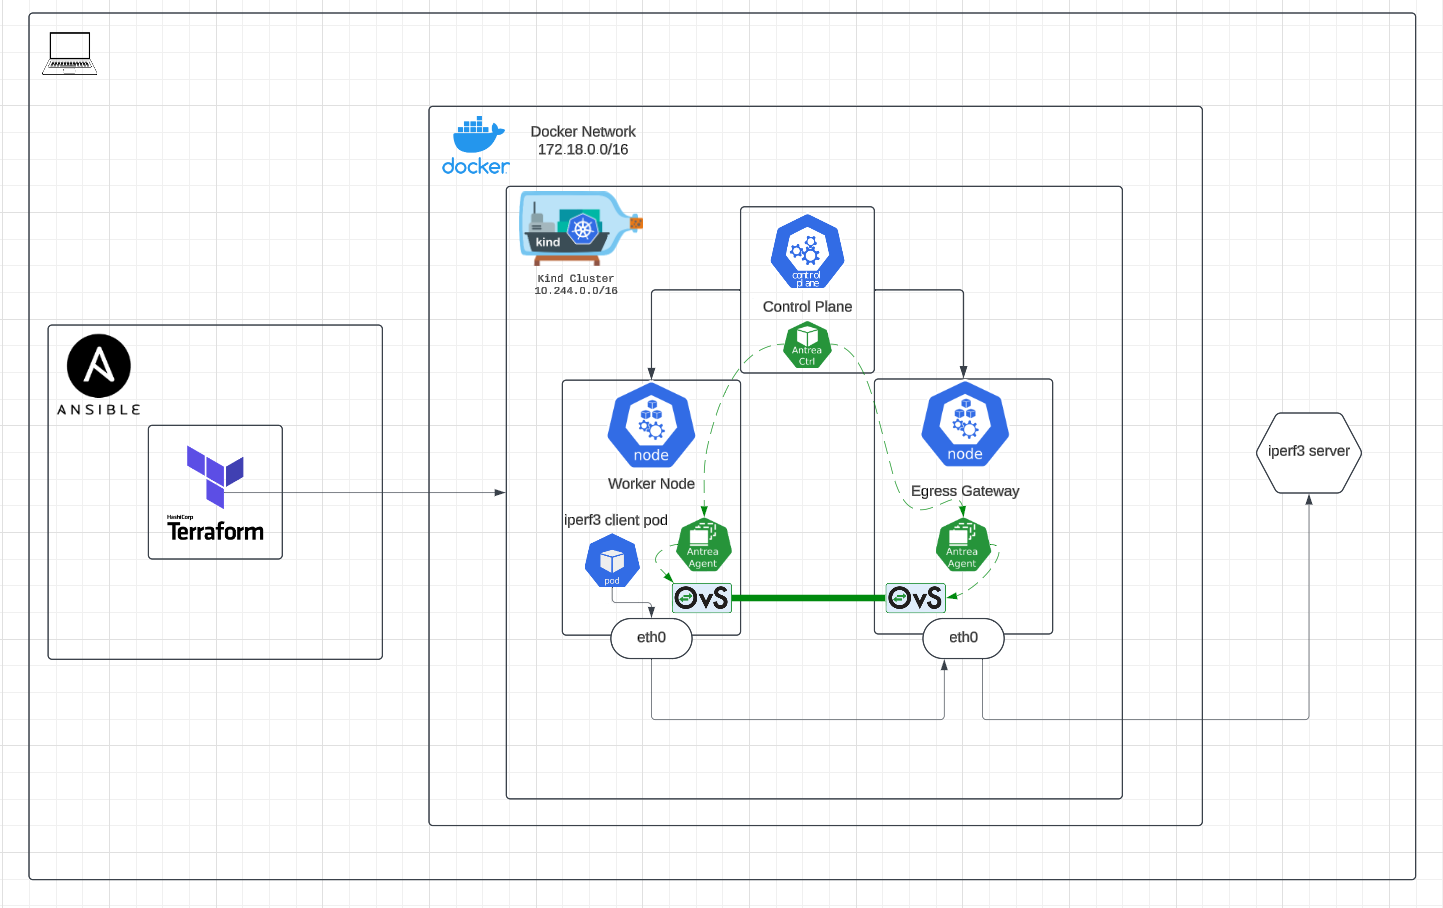
\includegraphics[width=1\columnwidth]{images/antrea_egress_gatateway_cluster.png}
  \caption{Antrea Egress Scenario infrastructure.}
  \label{fig:antreaEgressScenarioArch}
\end{figure}

Kubernetes cluster visible in figure~\ref{fig:antreaEgressScenarioArch} is provisioned on personal computer using Kind, and configured using Ansible and Terraform. The cluster consists of three nodes, a control plane, a worker node and an egress gateway, which are belonging to docker network. When role terraform\_run\_egress\_iperf begins its execution and created iperf3 Pod is ready the test begins, client using TCP protocol is sending data to server (outside cluster), which is routed through egress gateway. Iperf3 server discovers that traffic is incomming from egress gateway node (it sees IP address of Egress Gateway Node as a source), because traffic from the Pod is SNATed.
The iperf3 client sedns data packets using three-way handshake (TCP TODO CITE), after receiving acknowledgment from server, networking metrics are stored in its memory and at the end of the test, json file with gathered data is saved inside a Pod. The node exporter is constantly scraping the metrics, which are pulled by a Prometheus to its datbase. After the measurement is over, unformatted data is downloaded from prometheus and saved to csv file.

\begin{figure}[tbh]
  \centering
  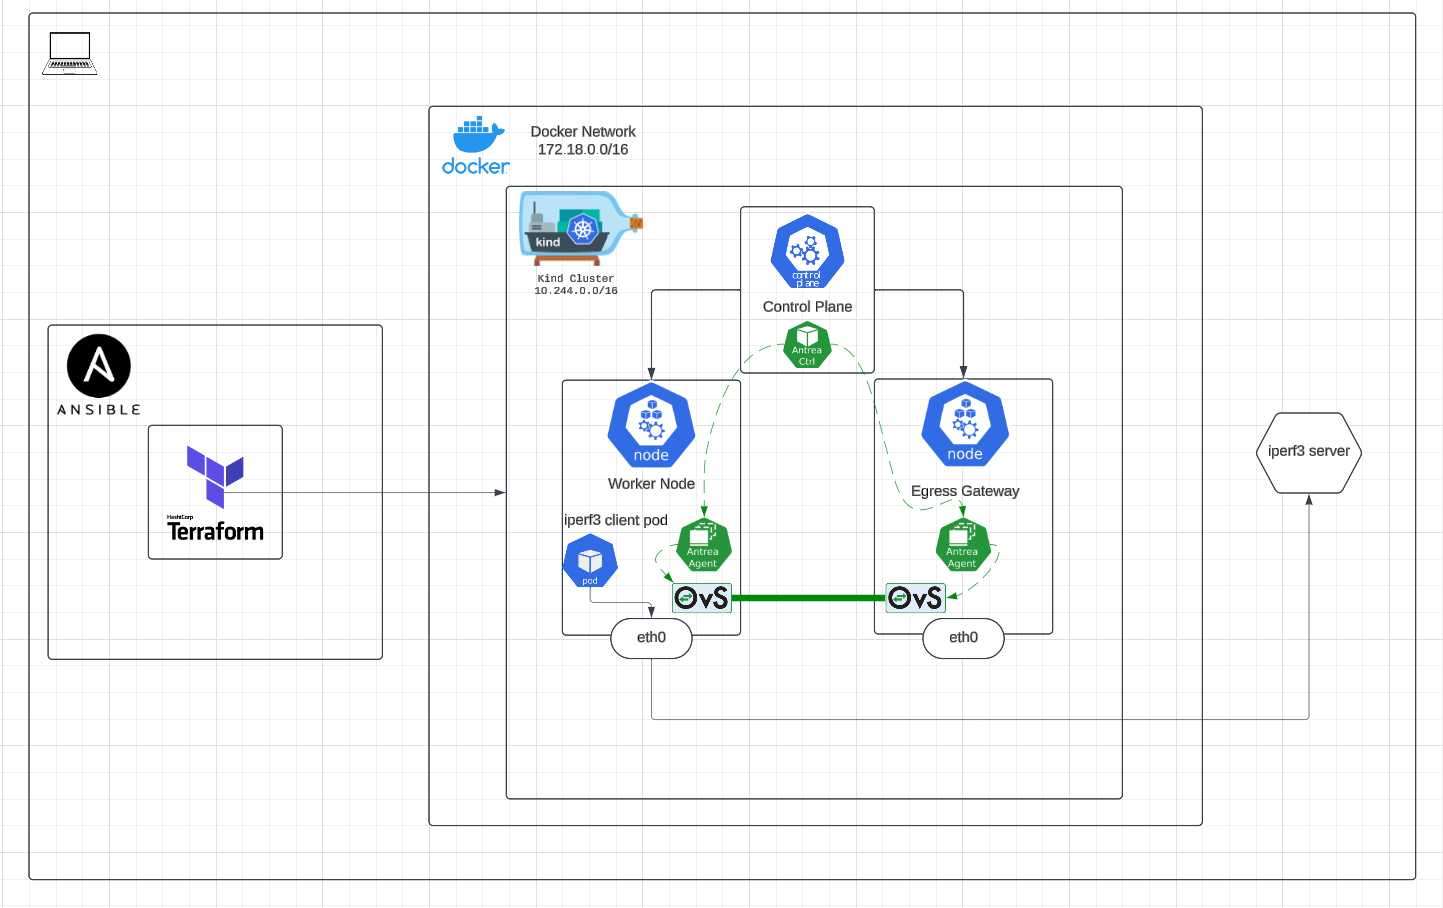
\includegraphics[width=1\columnwidth]{images/antrea_egress_no_gateway.png}
  \caption{Antrea Egress Scenario infrastructure without using Egrees Gateway.}
  \label{fig:antreaEgressNoGatewayScenarioArch}
\end{figure}

As seen on figure~\ref{fig:antreaEgressNoGatewayScenarioArch} the only difference is that, traffic initiated inside the iperf3 client pod is not leaving cluter through an Egress Gateway. This setup is designed to compare networking metrics and resource utilization with and without routing traffic through an Egress Gateway.

%---------------------------------------------------------------------------

\subsection{Cilium}
\label{sec:ciliumEgress}

The playbook for cilium is really similiar to the one which creates egress scenario using Antre CNI. The ansible roles are designed to be reused in different playbooks, the only differences are, CNI installation, Egress Gatewway deployment and in cilium desired node is labelled with egress-node=true. The infrastructure can be seen in figure~\ref{fig:ciliumEgressGatewayScenarioArch}.

\begin{figure}[tbh]
  \centering
  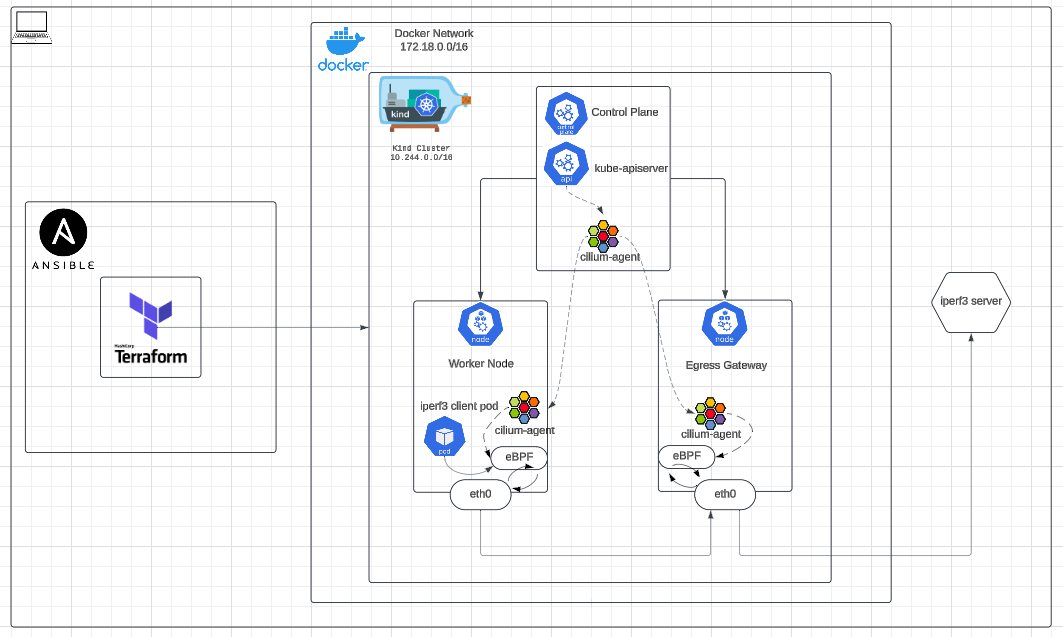
\includegraphics[width=1\columnwidth]{images/cilium_egress_gatateway_cluster.png}
  \caption{Cilium Egress Scenario infrastructure.}
  \label{fig:ciliumEgressGatewayScenarioArch}
\end{figure}
%---------------------------------------------------------------------------

\section{Ingress scenario implementation}
\label{sec:ingressImpl}

The ingress scenario evaluates the Antrea and Cilium Container Networking Plugins CPU and memory usage while using Gateway API in handling weighted traffic routing. The experiment involves using the Gateway API to route 40\% of incoming requests to one Pod and evaluating accuracy of traffic splitting by two different Gateway APIs. The test setup includes the k6 load testing tool running outside the Kubernetes cluster, generating traffic towards the Gateway API. The simulated traffic has four intensity levels by allocating different number of virtual users talking to the Gateway API. These are one, ten, houndred and tousand virtual users. The traffic is initiated using k6 tool, which runs inside container on personal computer. The network generator is performing HTTP request at Gatewy API and saves received response extracting Pod name to the text file (one per line). Having a list of responses containing names of two pods, accuracy of Gateway API traffic splitting is calculated. CPU and memory usage, is monitored with a Node Exporter during whole test and fetched at the end of scenario.


%---------------------------------------------------------------------------
\subsection{Cluster provisioning}
\label{sec:clusterProvisioning}

Creating a local cluster using Kind is a straightforward process, as described earlier. However, when setting up a Kubernetes cluster on Azure, the azurerm terraform provider must be configured properly to be authenticated with an azure account. The script shown on listing~\ref{lst:terraformScript} is responsible for creating Kubernetes cluster in Azure Services. It is important to choose appropriate location for cluster, define default node pool (virtual machine type and node count) and to get rid of default CNI by setting network\_plugin in network\_profile to "none" if different networking plugin is preffered \cite{AKS}.

\begin{listing}[htb]
  \centering
  \caption{Terraform Azure Kubernetes Service creation script \cite{AKS}.}
  \begin{minted}[gobble=4, frame=single, linenos, fontsize=\scriptsize]{hcl}
    resource "azurerm_resource_group" "rg" {
      location = var.resource_group_location
      name     = "rg${var.common_infix}"
    }

    resource "azurerm_kubernetes_cluster" "k8s" {
      location            = azurerm_resource_group.rg.location
      name                = "cluster${var.common_infix}"
      resource_group_name = azurerm_resource_group.rg.name
      dns_prefix          = "dns${var.common_infix}"

      identity {
        type = "SystemAssigned"
      }

      default_node_pool {
        name       = "agentpool"
        vm_size    = var.vm_type
        node_count = var.node_count
      }

      linux_profile {
        admin_username = var.username

        ssh_key {
          key_data = azapi_resource_action.ssh_public_key_gen.output.publicKey
        }
      }

      network_profile {
        network_plugin    = "none"
        load_balancer_sku = "standard"
      }
    }
  \end{minted}
  \label{lst:terraformScript}
\end{listing}


%---------------------------------------------------------------------------
\subsection{Antrea}
\label{sec:antreaIngressImpl}

The process of creating ingress scenario with Antrea CNI on Azure Kubernetes Services is fully automated showed on listing ~\ref{lst:antreaIngressPlaybook}. The script provisions an infrastructure seen on~\ref{fig:antreaIngressScenarioArch}. The steps in the scripts are: 


\begin{enumerate}
  \item create\_azure\_cluster -- runs terraform to provision infrastructure in the cloud and configures the local environment to allow kubectl to interact with the cluster
  \item install\_antrea -- installs Antrea CNI plugin
  \item wait\_until\_antrea\_installed -- waits until Antrea is installed
  \item install\_gateway\_api\_crd -- applys custom definiton resources, Gateway, GatewayClass, HTTPRoutes etc
  \item install\_nginx\_gateway\_fabric -- isntall NGINX Gateway Fabric using helm and waits util is fully installed
  \item deploy\_antrea\_ingress\_scenario -- deploys ingress scenario (echo Pods and Gateway API) using terraform
  \item monitoring -- enables monitoring with Node Exporter and Prometheus
  \item register\_gateway\_api\_ip -- registers api of Gateway API for k6 tool
  \item run\_k6 -- creates container with k6 which generates HTTP traffic acessing Gateway API
  \item scrap\_prometheus\_data -- downloads data about CPU and memory utilization
\end{enumerate}

\begin{listing}[H]
  \centering
  \caption{Kind config used in both scenarios \cite{KindConfig}.}
  \begin{minted}[gobble=4, frame=single, linenos, fontsize=\scriptsize]{yaml}
    - name: Create antrea ingres scenario with gateway api
      hosts: "{{ target | default('localhost') }}"
      vars_files:
        - ./vars/antrea.yml
        - ./vars/cloud.yml
        - ./vars/common.yml
        - ./vars/traffic_splitting.yml

      roles:
        - create_azure_cluster
        - install_antrea_cloud
        - wait_until_antrea_installed
        - install_gateway_crd
        - install_nginx_gateway
        - deploy_antrea_ingress_scenario
        - monitoring
        - register_gateway_api_ip
        - run_k6
        - scrap_prometheus_data
  \end{minted}
  \label{lst:antreaIngressPlaybook}
\end{listing}


\begin{figure}[tbh]
  \centering
  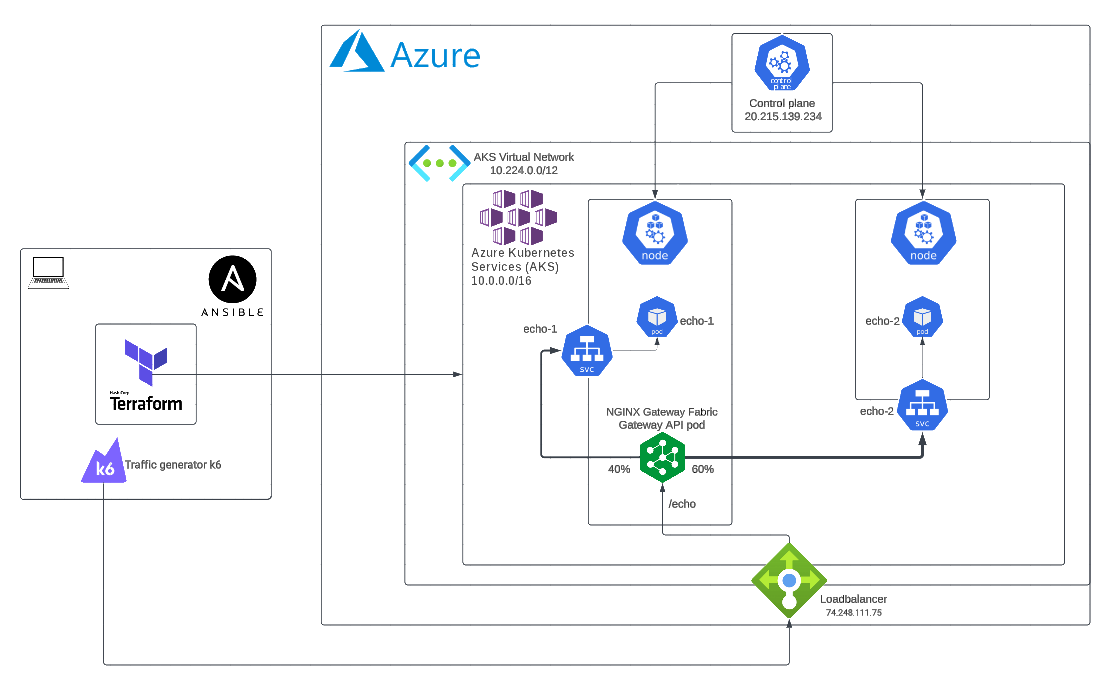
\includegraphics[width=1\columnwidth]{images/antrea_cloud_traffic_splitting.png}
  \caption{Antrea Ingress Scenario infrastructure.}
  \label{fig:antreaIngressScenarioArch}
\end{figure}

%---------------------------------------------------------------------------
\subsection{Cilium}
\label{sec:ciliumIngressImpl}

The ingress scenario with the Cilium CNI plugin does not need to install the NGINX Gateway Fabric, as it utilizes its own built-in implementation.



\begin{figure}[H]
  \centering
  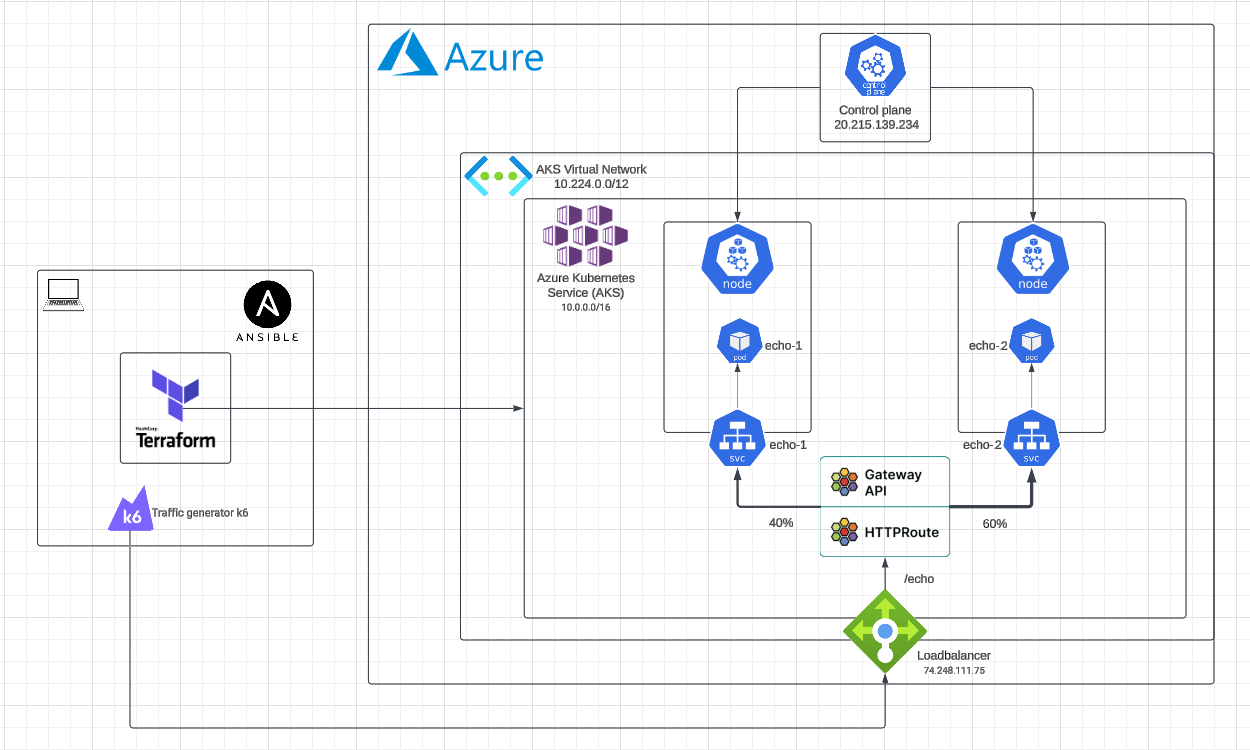
\includegraphics[width=1\columnwidth]{images/cilium_cloud_traffic_splitting.png}
  \caption{Cilium Ingress Scenario infrastructure.}
  \label{fig:ciliumIngressScenarioArch}
\end{figure}
%---------------------------------------------------------------------------

\subsection{The differences between cloud and local runs}
\label{sec:diff}

\subsubsection{Control plane}
\label{sec:cplaneDiff}

In the local environment, the control plane node is created in the same way as the worker nodes, running as a container. However, when using NGINX with the Antrea CNI, the NGINX Gateway Fabric pod is deployed on a separate control plane node. This setup allows the routing of traffic between two different nodes, ensuring that traffic is always leaving the node. In contrast, when using AKS (Azure Kubernetes Service), the control plane is not part of the node pool; it is a separate managed service outside of the node pool, providing a more distinct separation between the control plane and worker nodes. This architectural difference can affect the measurements (in comparison to local stack), as resource utiliazation of the control plane node is not gathered.

\subsubsection{Client traffic generator}
\label{sec:clientServerDiff}

In the cloud setup, the client running on a personal computer generates HTTP requests to the public Gateway API IP address exposed by Azure Cloud. Resource utilization within the cluster is exclusively used by the cluster itself, not by the client. However when running local stack, the client is part of a laptop on which cluster is running, what might influence measurements.
